% !TEX TS-program = pdflatex
% !TEX encoding = UTF-8 Unicode

% This is a simple template for a LaTeX document using the "article" class.
% See "book", "report", "letter" for other types of document.

\documentclass[11pt]{scrreprt} % use larger type; default would be 10pt

\usepackage[utf8]{inputenc} % set input encoding (not needed with XeLaTeX)
\usepackage{german}
%%% Examples of Article customizations
% These packages are optional, depending whether you want the features they provide.
% See the LaTeX Companion or other references for full information.

%%% PAGE DIMENSIONS
\usepackage{geometry} % to change the page dimensions
\geometry{a4paper} % or letterpaper (US) or a5paper or....
% \geometry{margins=2in} % for example, change the margins to 2 inches all round
% \geometry{landscape} % set up the page for landscape
%   read geometry.pdf for detailed page layout information

\usepackage{graphicx} % support the \includegraphics command and options

% \usepackage[parfill]{parskip} % Activate to begin paragraphs with an empty line rather than an indent

%%% PACKAGES
\usepackage{booktabs} % for much better looking tables
\usepackage{array} % for better arrays (eg matrices) in maths
\usepackage{paralist} % very flexible & customisable lists (eg. enumerate/itemize, etc.)
\usepackage{verbatim} % adds environment for commenting out blocks of text & for better verbatim
\usepackage{subfig} % make it possible to include more than one captioned figure/table in a single float
\usepackage{german}
\usepackage{url}
\usepackage{hyperref}
\usepackage{amsfonts}
\usepackage{amsmath}
\usepackage{amsthm}
\usepackage{listings}
% These packages are all incorporated in the memoir class to one degree or another...

\usepackage{listings}
\usepackage{color}
\definecolor{lightgray}{rgb}{.9,.9,.9}
\definecolor{darkgray}{rgb}{.4,.4,.4}
\definecolor{purple}{rgb}{0.65, 0.12, 0.82}

\lstset{
   language=C++,
   backgroundcolor=\color{lightgray},
   extendedchars=true,
   basicstyle=\footnotesize\ttfamily,
   showstringspaces=false,
   showspaces=false,
   %numbers=left,
   numberstyle=\footnotesize,
   numbersep=9pt,
   tabsize=2,
   breaklines=true,
   showtabs=false,
   captionpos=b
}

%%% HEADERS & FOOTERS
\usepackage{fancyhdr} % This should be set AFTER setting up the page geometry
\pagestyle{fancy} % options: empty , plain , fancy
\renewcommand{\headrulewidth}{0pt} % customise the layout...
\lhead{}\chead{}\rhead{}
\lfoot{}\cfoot{\thepage}\rfoot{}

%%% SECTION TITLE APPEARANCE
\usepackage{sectsty}
\allsectionsfont{\sffamily\mdseries\upshape} % (See the fntguide.pdf for font help)
% (This matches ConTeXt defaults)

%%% ToC (table of contents) APPEARANCE
\usepackage[nottoc,notlof,notlot]{tocbibind} % Put the bibliography in the ToC
\usepackage[titles,subfigure]{tocloft} % Alter the style of the Table of Contents
\renewcommand{\cftsecfont}{\rmfamily\mdseries\upshape}
\renewcommand{\cftsecpagefont}{\rmfamily\mdseries\upshape} % No bold!

%%% END Article customizations

%%% The "real" document content comes below...

\theoremstyle{definition}
\newtheorem*{beisp}{Beispiel}
\newtheorem{definition}{Definition}
\newtheorem*{bemerkung}{Bemerkung}

\title{Paralleles Lesen und Schreiben von farbigen 2D-Barcodes mit MPI}
\subtitle{Seminar Wissenschaftliches Rechnen \\ ZHAW, Zürich}
\author{Florian Lüthi\footnote{\url{luethifl@students.zhaw.ch}}}
%\date{ZHAW (Zürich), 5. Juni 2013} % Activate to display a given date or no date (if empty),
         % otherwise the current date is printed 

\begin{document}
\maketitle

\tableofcontents

\chapter{Einleitung}

Diese Arbeit beschäftigt sich mit der von Md. Mashud Rana, M. E. Kawsar, M. E. Rabbani, S. M. M. Rashid und K. E. U. Ahmed vorgeschlagenen Methode des Lesens und Schreibens von farbigen zweidimensionalen Barcodes mit hoher Datenkapazität \cite{paper}.

Sie beschreibt diese Methode, zeigt eine mögliche Umsetzung des Verfahrens in {\tt C++} mit Parallelisierung mittels {\tt MPI}, und macht eine quantitative Analyse der Implementation in Bezug auf die Performance. Zu guter Letzt zieht sie ein Fazit und überlegt sich den Sinn der angewandten Methode.

Zur Arbeit gehören dieses Dokument sowie die Beispielimplementation. Beides kann von \url{https://github.com/foyan/ColorizedBarCodec} bezogen werden.

Der Autor bedankt sich bei Dr. Alexander Herrigel für die Durchführung des Seminars.

\chapter{Einführung in das Thema}

\section{Existierende Technologien}

Seit den 1970er-Jahren \cite{wiki:barcode} sind Barcodes aus Logistikbetrieben, Supermärkten etc. nicht mehr wegzudenken. Sie bilden das Rückgrat der automatisierten Warenbewirtschaftung. Das Scanning von eindimensionalen Barcodes wie in Abbildung \ref{fig:onedbarcode} ist milliardenfach erprobt und in der Entwicklung eigentlich abgeschlossen.

\begin{figure}
\caption{Eindimensionaler Barcode (Quelle: Wikipedia)}
\label{fig:onedbarcode}
\begin{center}
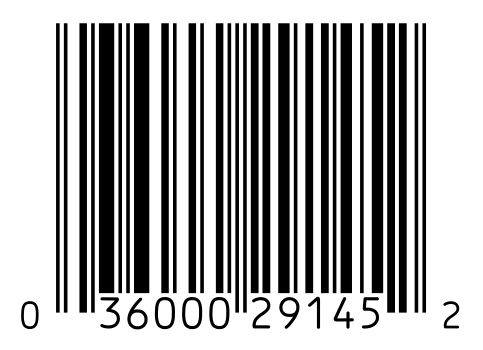
\includegraphics[scale=0.4]{biltli/onedbarcode.png}
\end{center}
\end{figure}

Die Informationsdichte von eindimensionalen Barcodes ist aber sehr beschränkt. Beispielsweise erlaubt die eindimensionale Symbologie UPC-A maximal eine Billion eindeutiger Barcodes \cite{wiki:upc}, was gemäss
\[
\log_2 10^{12} = 39.863\dots
\]
einer maximalen Kapazität von weniger als 5 Bytes entspricht.

Aus diesem Grund wurden mit dem Aufkommen von billigen und sehr akkuraten Kameras in mobilen Devices zweidimensionale Symbologien entwickelt, welche es zumindest erlauben, ganze URLs von Webseiten oder ähnliches zu codieren. Google beispielsweise vermarktet den in Abbildung \ref{fig:qr} ersichtlichen, ursprünglich von Toyota entwickelten {\it Quick Response} Code (QR) \cite{wiki:qr}. Dieser erlaubt es immerhin, maximal 2953 Bytes zu codieren \cite{wiki:qr}.


\begin{figure}
\caption{QR Code (Quelle: Wikipedia)}
\label{fig:qr}
\begin{center}

\includegraphics[scale=0.4]{biltli/qr.png}
\end{center}
\end{figure}

Um die Kapazität weiter zu steigern, ist es nötig, eine dritte Dimension einzuführen. Weil aber Hologramme und 3D-Kameras noch nicht marktreif sind, liegt es nahe, die dritte Dimension als Farbe zu codieren. Microsoft geht in seiner Barcode-Technologie {\it High Capacity Color Barcode (HCCB)} seit 2007 \cite{wiki:hccb} genau diesen Weg \cite{ms:hccb}. Ein Beispiel ist in Abbildung \ref{fig:hccb} abgebildet. Die maximale Kapazität von HCCB kann nicht genau genannt werden, weil die Barcodes keine definierte Grösse und Skalierung haben. Labortests scheinen aber gezeigt zu haben, dass es möglich ist, circa 2000 Bytes auf eine Fläche zu codieren, welche nicht viel grösser als eine Ein-Cent-Münze ist. Diese Fläche scheint sich mit einem 600-dpi-Laserdrucker herstellen zu lassen \cite{ms:hccb}.


\begin{figure}
\caption{High Capacity Color Barcode (Quelle: Wikipedia)}
\label{fig:hccb}
\begin{center}

\includegraphics[scale=0.4]{biltli/hccb.png}
\end{center}
\end{figure}

\section{Vorgeschlagene Methode}

Rana, Kawsar, Rabbani, Rashid und Achmed schlagen nun eine Methode vor, welche sich durch eine hohe Kapazität sowie ein sehr schnelles Leseverfahren auszeichnen soll \cite{paper}. Die grundlegenden Eckwerte sind die folgenden:

\begin{itemize}
\item Es werden 16 verschiedene Farben verwendet. Jede dieser Farben wird bijektiv einer Sequenz aus 4 Bits (Nibbles) zugeordnet (siehe Tabelle \ref{tab:colormap}, \cite{paper}).

\item Jedes Byte wird auf ein Zeichen abgebildet (siehe \cite{paper}).

\item Die Fläche des Barcodes wird in ein $102 \times 100$ Zellen fassendes Raster aufgeteilt (im folgenden als Pixel bezeichnet). Bei einer angenommenen realen Grösse des Barcodes von $1.5 \times 1.15$ Zoll \cite{paper} ergibt sich daraus eine horizontale Auflösung von 68 DPI und eine vertikale Auflösung von 87 DPI.

\item Jeweils 6 benachbarte Pixel in einem $3 \times 2$-Feld codieren nun ein Byte, wobei ein ein vertikal gespiegeltes {\tt L} für den ersten Nibble und ein horizontal gespiegeltes {\tt L} für den zweiten Nibble entstehen (Abbildung \ref{fig:onebyte}). Über die Reihenfolge der Wertigkeit der Nibbles wird keine Vorschrift gemacht -- die abgebildete Rot/Grün-Kombination könnte also sowohl als {\tt 0000 0001} $=1$ als auch als {\tt 0001 0000} $=16$ interpretiert werden.

\end{itemize}

Weil je nach codierter Information die Länge der Codierung variiert, schlägt \cite{paper} vor, die ersten Nibbles als Header zu reservieren\footnote{Bezüglich der Länge des Headers werden in \cite{paper} widersprüchliche Aussagen gemacht. Der Text reserviert die ersten 12 Pixel, was einer Länge von 2 Bytes entsprechen würde, wogegen die dazugehörige Abbildung eine Länge von 9 Pixeln kolportiert, was einer Länge von 1.5 Bytes entsprechen würde. Im Nachfolgenden wird darum eine Headerlänge von 2 Bytes angenommen.}, welche als Information nur die Länge der nachfolgenden Informationen enthalten.

Die maximale Kapazität des Barcodes ist darum
\[
C = \frac{102 \operatorname{px} \cdot 100 \operatorname {px}}{6 \operatorname{px}^2 / \operatorname{byte}} - 2 \operatorname{bytes} = 1698 \operatorname{bytes}.
\]

\begin{table}
\caption{Zuordnung der Farben zu den Nibbles}
\label{tab:colormap}
\begin{center}
\begin{tabular}{rrl}
\toprule
Wert & Nibble (binär) & RGB-Wert \\
\midrule
0 & {\tt 0000} & {\tt rgb(255, 000, 000)} \\
1 & {\tt 0001} & {\tt rgb(000, 128, 000)} \\
2 & {\tt 0010} & {\tt rgb(000, 000, 025)} \\
3 & {\tt 0011} & {\tt rgb(165, 042, 042)} \\
4 & {\tt 0100} & {\tt rgb(128, 000, 000)} \\
5 & {\tt 0101} & {\tt rgb(100, 149, 237)} \\
6 & {\tt 0110} & {\tt rgb(255, 165, 000)} \\
7 & {\tt 0111} & {\tt rgb(255, 255, 000)} \\
8 & {\tt 1000} & {\tt rgb(238, 130, 238)} \\
9 & {\tt 1001} & {\tt rgb(128, 128, 128)} \\
10 & {\tt 1010} & {\tt rgb(000, 000, 128)} \\
11 & {\tt 1011} & {\tt rgb(000, 000, 000)} \\
12 & {\tt 1100} & {\tt rgb(173, 255, 047)} \\
13 & {\tt 1101} & {\tt rgb(138, 043, 226)} \\
14 & {\tt 1110} & {\tt rgb(128, 000, 128)} \\
15 & {\tt 1111} & {\tt rgb(095, 158, 160)} \\

\bottomrule
\end{tabular}
\end{center}
\end{table}


\begin{figure}
\caption{Ein Byte in der vorgeschlagenen Methodik}
\label{fig:onebyte}
\begin{center}

\includegraphics[scale=10]{biltli/onebyte.png}
\end{center}
\end{figure}


\chapter{Randbedingungen}

Das beschriebene, untersuchte und implementierte Verfahren \cite{paper} impliziert in sich schon mehrere Randbedingungen beziehungsweise Einschränkungen bezüglich allgemeiner Brauchbarkeit, deren Diskussion in Kapitel \ref{sec:bewertung} aufgenommen wird.

Vorauseilend kann schon einmal gesagt werden, dass in Punkto Kapazitätserweiterung kein Fortschritt erreicht wird, weil der {\it QR}-Code intrinsisch schon eine höhere Kapazität aufweist, ohne allerdings den Vorteil der Farbdimension für sich reklamieren zu können.

Diese Arbeit hat darum explizit nicht das Ziel, eine wirkliche Alternative oder eine sinnvolle Entwicklungsrichtung in Sachen Barcodes aufzuzeigen. Sie ist eher als Schulbeispiel zur Umsetzung einer einfachen Algorithmik mittels Parallelisierung zu verstehen.

\chapter{Auswahl der Testdaten für die Arbeit}

Die Aufgabe des Algorithmus ist, Text in ein Bild umzuformen und wieder zurück. Dementsprechend werden drei Texte ausgewählt, welche zusammen mit ihren entsprechenden Barcodes die Testdaten bilden:

\begin{enumerate}
\item Um den minimalen Fall zu testen, wird der leere Text ausgewählt. Der korrespondierende Barcode ist in Abbildung \ref{test:leer} zu sehen.
\item Um einen durchschnittlichen Fall zu testen, wird die Definition der Aufklärung von Immanuel Kant aus dessen Essay {\it Beantwortung der Frage: Was ist Aufklärung?} von 1784 \cite{kant} verwendet:

\begin{quote}
Aufklärung ist der Ausgang des Menschen aus seiner selbstverschuldeten Unmündigkeit. Unmündigkeit ist das Unvermögen, sich seines Verstandes ohne Leitung eines anderen zu bedienen. Selbstverschuldet ist diese Unmündigkeit, wenn die Ursache derselben nicht am Mangel des Verstandes, sondern der Entschliessung und des Muthes liegt, sich seiner ohne Leitung eines anderen zu bedienen. Sapere aude! Habe Muth, dich deines eigenen Verstandes zu bedienen! ist also der Wahlspruch der Aufklärung. \cite{wiki:kant}

\end{quote}
Die Länge dieses Textes beträgt (nach Ersetzung von {\tt ß} durch {\tt ss} sowie dem Einfügen einiger Zeilenumbrüche wegen der besseren Lesbarkeit) exakt 500 Bytes, was einer Ausnutzung der Kapazität von 29.4 Prozent entspricht. Der korrespondierende Barcode ist in Abbildung \ref{test:kant} zu sehen.

\item Um den maximalen Fall zu testen, wird ebendieser Text solange wiederholt, bis die maximale Kapazität erreicht ist. Der korrespondierende Barcode ist in Abbildung \ref{test:kantkant} zu sehen.

\begin{figure}
\caption{Der leere Barcode}
\label{test:leer}
\begin{center}
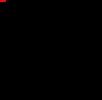
\includegraphics[scale=1.4]{../leer.png}
\end{center}
\end{figure}
\begin{figure}
\caption{Die Antwort auf die Frage: Was ist Aufklärung? als Barcode}
\label{test:kant}
\begin{center}
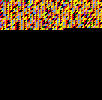
\includegraphics[scale=1.4]{../kant.png}
\end{center}
\end{figure}
\begin{figure}
\caption{Möglichst viel Kant in einem Barcode}
\label{test:kantkant}
\begin{center}
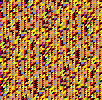
\includegraphics[scale=1.4]{../kantkant.png}
\end{center}
\end{figure}


\end{enumerate}

\chapter{Algorithmische Beschreibung des Verfahrens}

\section{Codieren des Barcodes}

Der folgende Algorithmus beschreibt den Codierungsvorgang eines Barcodes (seien {\tt text} der zu codierende Text, {\tt width} und {\tt height} die Breite und Höhe des Barcodes, {\tt color()} die Nibble-Farbe-Abbildung und {\tt bc} der resultierende Barcode):

\begin{verbatim}
algo encode:
    for i in [0..|text|-1]:
        var x = (i*3) mod width
        var y = (i*3) / width * 2
        bc[x, y] = bc[x+1, y] = bc[x, y+1] = color(text[i].low)
        bc[x+1, y+1] = bc[x+2, y+1] = bc[x+2, y] = color(text[i].high)
\end{verbatim}

\section{Decodieren des Barcodes}

Der folgende Algorithmus beschreibt den Decodierungsvorgang eines Barcodes (seien {\tt bc} der zu dcodierende Barcode, {\tt width} und {\tt height} die Breite und Höhe des Barcodes, {\tt nibble()} die Farbe-Nibble-Abbildung, {\tt detect\_color()} der weiter unten beschriebene Error-Correction-Algorithmus und {\tt text} der resultierende Text):

\begin{verbatim}
algo decode:
    for (y, x) in [0..height-1] x [0..width-1] step (2, 3):
        var c1 = detect_color(bc[x, y], bc[x+1, y], bc[x, y+1])
        var c2 = detect_color(bc[x+1, y+1], bc[x+2, y+1], bc[x+2, y])
        text.append(nibble(c2) nibble(c1))
\end{verbatim}

\section{Error Correction}

Die in \cite{paper} vorgeschlagene probabilistische Error Detection und Correction-Methode funktioniert folgendermassen (seien {\tt m}, {\tt s1}, {\tt s2} die Farben an den entsprechenden Position innerhalb des {\tt L}s):

\begin{verbatim}
algo detect_color:
    if m = s1:
        return m
    if s1 = s2:
        return s1
    return s2
\end{verbatim}

\section{Bewertung des Verfahrens}
\label{sec:bewertung}

An der von \cite{paper} proklamierten Einfachheit und {\tt computational efficiency} des Verfahrens gibt es gar nichts auszusetzen: Unter der gültigen Annahme, dass sowohl {\tt color()} als auch {\tt nibble} als reine Hashtable-Lookup-Funktionen eine asymptotische Laufzeitkomplexität von (sei $x$ der Text oder der Barcode):
\[
f(x) \in \mathcal{O}(1)
\]
haben, beträgt die asymptotische Laufzeitkomplexität sowohl von {\tt encode} wie auch von {\tt decode}
\[
f(x) \in \mathcal{O}(|x|).
\]

Durch diese verfahrenstechnische Effizienz werden allerdings mehrere Mängel in Kauf genommen, die sich schnurstracks auf die Effektivität des Verfahrens auswirken:

\begin{enumerate}
\item Der Platz, den ein Byte an Information einnehmen kann, ist steht immer in einem festen Verhältnis zur gesamten Grösse des Barcodes (nämlich 6 Pixel). Dadurch hat ein resultierender Barcode immer automatisch die maximal mögliche Informationsdichte (was in den Abbildungen \ref{test:leer} und \ref{test:kant} sehr schön ersichtlich ist: da die zu codierenden Informationen weniger sind als die maximal mögliche Kapazität, bleibt ein geographisch zusammenhängender Teil des Barcodes ungenutzt, sprich schwarz).

Reifere Verfahren nutzen hingegen immer den ganzen zur Verfügung stehenden Platz, indem sie dynamisch die Informationsdichte ausdünnen. Dadurch vergrössern sie die Toleranz gegenüber der Ungenauigkeit während des Lesens (welche in der Realität bei Scans oder Fotografien natürlich immer da ist).

Das Verfahren könnte in dieser Hinsicht natürlich verbessert werden, weil die Länge der Information aus dem Header ersichtlich ist. Daraus liesse sich die physische Grösse eines Pixels berechnen. Allerdings ist der Header selber als mehrere Pixel codiert. Deshalb müsste trotzdem ein Verfahren implementiert werden, welches quasi die Grösse eines Pixels rekonstruiert -- was sich natürlich saftig in einer höheren Gesamtkomplexität niederschlagen würde.

\item Das Verfahren beinhaltet keinerlei Paritätsprüfung der Daten. Abgesehen davon, dass die Farbwerte der gescannten Pixel exakt denjenigen in Tabelle \ref{tab:colormap} entsprechen müssen (was bei einem Scan in der Realität nur schon wegen den variierenden Lichtverhältnissen wegen sowieso utopisch ist), würde der als {\tt Error Correction und Detection}-Algorithmus \cite{paper} kolportierte Algorithmus {\tt detect\_color()} bei drei verschiedenen (und gemäss Tabelle \ref{tab:colormap} gültigen!) Farbwerten unreflektierterweise einfach den letzten der drei Werte als richtig erachten.

Das Verfahren könnte verbessert werden, indem es um eine typische Paritätsprüfungsmethode ergänzt werden würde -- beispielsweise {\tt CRC}. Die aymptotische Komplexität würde nicht darunter leiden; der Seiteneffekt wäre allerdings, dass nicht mehr zwei Nibbles ein ganzes Byte ergeben würden und darum das Mapping zwischen Bytes und Zeichen massiv komplizierter würde.

\end{enumerate}

\chapter{Analyse, Design und Implementierung des Verfahrens}

\section{Parallelisierung}

Die Codierungs- und Decodierungs-Algorithmen selber sind einigermassen simpel. Der parallelisierbare Teil der beiden Algorithmen besteht allerdings nur aus dem Mapping-Teil, da der zu codierende Text oder das zu decodierende Bild natürlich nur auf jeweils einem Node des Clusters vorliegen.

Da der Codierungs-Algorithmus mehr oder weniger die Umkehrfunktion des Decodierungs-Algorithmus ist, kann die Infrastruktur der beiden geteilt werden. Dadurch ist es möglich, die Parallelisierung vollständig aus den Algorithmen zu extrahieren: Sei {\tt algo} einer der beiden besprochenen Algorithmen mit diesen Teilalgorithmen:
\begin{itemize}
\item {\tt init}
\item {\tt get\_sliced\_input}
\item {\tt process\_slice}
\item {\tt collect\_slice}
\item {\tt finalize},
\end{itemize}

dann sieht die parallelisierte Ausführung von {\tt algo} auf dem Master-Node folgendermassen aus:

\begin{verbatim}
algo.init()
for each slave node:
    var in = get_sliced_input(slave)
    invoke_slave(in)
var my_in = get_my_input()
algo.process_slice(my_input)
result += algo.collect_slice(my_input)
for each slave node:
    result += algo.collect_slice(slave)
algo.finalize()
\end{verbatim}

Die parallelisierte Ausführung auf einem Slave-Node besteht im Wesentlichen aus der Ausführung von {\tt algo.process\_slice()}.

Weil die Ausführung der Parallelisierung nun nichts mehr mit dem Ausführen der Algorithmen zu tun hat, kann nun natürlich das Strategy-Pattern angewandt werden, um die Ausführungen austauschbar zu machen. Im folgenden ist der Code der Methode {\tt task\_runner\_factory::create\_task\_runner} abgebildet, welche anhand des zweiten Kommandozeilenparameters entweder einen {\tt MPI}- oder einen simplen nichtparallelisierten {\tt task\_runner} herstellt:

\begin{lstlisting}
task_runner* task_runner_factory::create_task_runner(int argc, char* argv[]) {

	if (argc > 2 && strcmp(argv[2], "mpi") == 0) {
		return new mpi_task_runner();
	}

	return new simple_task_runner();

}
\end{lstlisting}

\section{Kommunikation der Nodes}

Damit die Algorithmen über einen Strang geschlagen werden können, müssen sie von einer gemeinsamen Basisklasse ableiten -- {\tt task}:

\begin{lstlisting}
class task {

public:
	virtual void init(int argc, char* argv[]) = 0;
	virtual void* get_sliced_input(int slice_index, int slice_count) = 0;
	virtual void* process_slice(void* input) = 0;
	virtual void collect_slice(void* slice, int slice_index, int slice_count) = 0;
	virtual void finalize() = 0;

	virtual void pack_input(pack&, void*) = 0;
	virtual void pack_output(pack&, void*) = 0;
	virtual void* unpack_input(pack&) = 0;
	virtual void* unpack_output(pack&) = 0;

	virtual ~task() { }
};

\end{lstlisting}

Damit der operierende {\tt task\_runner} nicht wissen muss, welche Datentypen er in der {\tt MPI}-World herumschickt (und die Basisklasse dies natürlich noch weniger weiss), funktioniert die In-Process-Kommunikation über {\tt void}-Pointer, wovon die konkreten {\tt task}s die korrekten (und nur für sie selber relevanten) Typen durch Casting zurückgewinnen können.

Ein Problem bleibt aber: Die verwendete {\tt boost\_serialization}-Library kann nur bekannte Typen serialisieren. Aus diesem Grund gibt es die {\tt pack}-Klasse, welche ein neutrales Paket machen kann, je nachdem ob {\tt string}s oder Pixel verschickt werden sollen:

\begin{lstlisting}
class pack {

public:
	string Str;
	vector<pair<rgb, rgb>> Pixels;

};

namespace boost {
	namespace serialization {

		template<typename Archive>
		void serialize (Archive& ar, pack& r, const unsigned int version) {
			ar & r.Str;
			ar & r.Pixels;
		}

	}
}
\end{lstlisting}

Die verschiedenen {\tt (un)pack\_*}-Methoden der einzelnen {\tt task}s werden dann vom {\tt task\_runner} entsprechend an der richtigen Stelle aufgerufen, um die Pakete entsprechend vor- oder nachzubereiten.

\section{Mapping}

Das Mapping von Farben zu Nibbles ist bijektiv, ergo braucht es für die Implementation eine bidirektionale {\tt map<>}\footnote{Auf ein explizites Mapping von Bytes zu Zeichen wie in \cite{paper} vorgeschlagen wurde verzichtet -- es scheint keinen sinnvollen Grund zu geben, in dieser Beziehung nicht die normale {\tt ASCII}-Codierung zu verwenden.}. In {\tt boost} wird man mit der {\tt bimap<>} natürlich fündig. Da diese Map von {\tt unsigned short} zur benutzerdefinierten Klasse {\tt rgb} abbildet und wieder zurück, muss eine natürliche Ordnung auf {\tt rgb} implementiert werden, damit {\tt bimap<>} die Eindeutigkeit garantieren kann. Dies wird über die Spezialisierung des Templates {\tt std::less<>} gelöst:
\begin{lstlisting}
namespace std {

	template<> struct less<rgb> : binary_function<rgb, rgb, bool> {
		bool operator() (const rgb& a, const rgb& b) const {
			if (a.r() < b.r()) {
				return true;
			}
			if (a.r() > b.r()) {
				return false;
			}
			if (a.g() < b.g()) {
				return true;
			}
			if (a.g() > b.g()) {
				return false;
			}
			return a.b() < b.b();
		}
	};

}
\end{lstlisting}

\section{Design-technische Übersicht}

Der Rest der Implementation ist eigentlich Schema F -- die besprochenen Algorithmen werden mehr oder weniger 1:1 implementiert, das Übrige das Bemühen von {\tt libpng} für IO mit dem Bild und das Zershreddern und Zusammenführen von {\tt string}s und {\tt vector<>}s. Stellvertretend illustriert Abbildung \ref{fig:arch} die Klassenarchitektur der Implementation.

\begin{figure}
\caption{Architektur}
\label{fig:arch}
\begin{center}
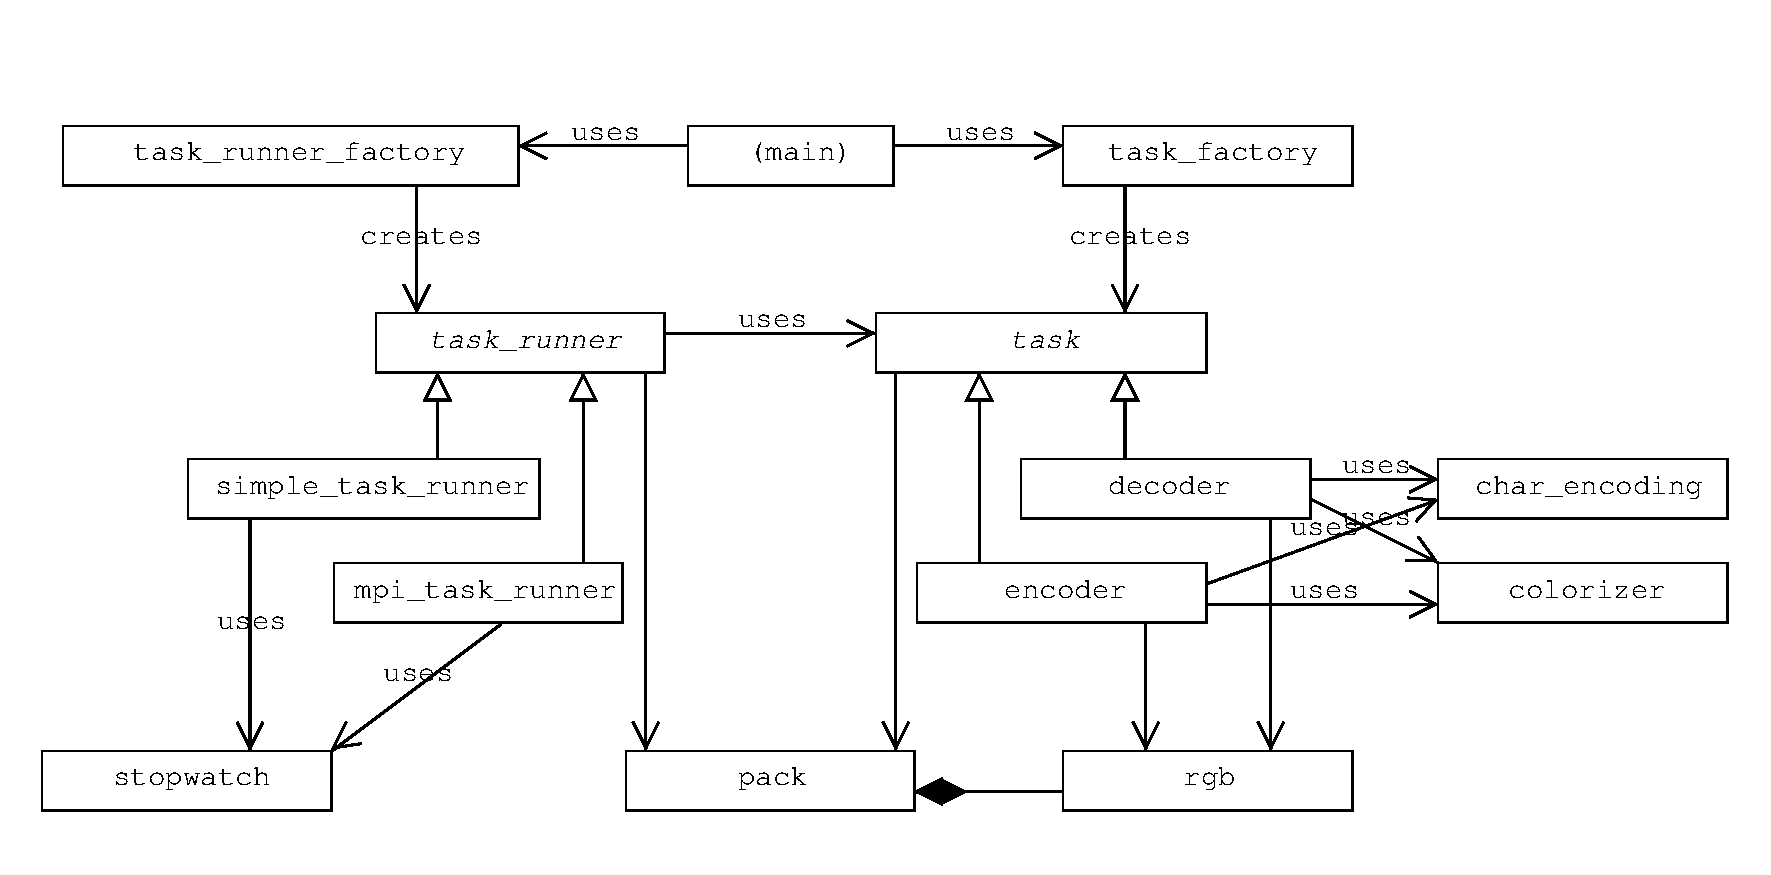
\includegraphics[scale=0.5]{biltli/arch.pdf}
\end{center}
\end{figure}

\chapter{Vergleich der Performancezeiten für ein, zwei oder mehrere CPU-Cores}

In Tabelle \ref{tab:perf} sind die durchschnittlichen Ausführungszeiten pro Testfall (minimal, durchschnittlich und maximal), Algorithmus und Anzahl Cores angegeben. Die Zeiten sind in Millisekunden, und es wurden jeweils fünf Ausführungen durchgeführt.

Das Tests wurden auf einem virtuellen Debian Wheezy mit 1 GB RAM und 4 vom Hostbetriebssystem (Windows 8) zugewiesenen Prozessorkernen durchgeführt.

Es sticht ins Auge, dass die Ausführungszeit besser ist, je {\it weniger} parallelisiert wird. Dies kann dadurch erklärt werden, dass der parallelisierbare Teil des Verfahrens trivial ist und gegenüber dem Kommunikations-Overhead sich praktisch in Nichts auflöst.

Der notorisch bessere Performance von {\tt decode} gegenüber {\tt encode} lässt sich dadurch erklären, dass das Schreiben eines {\tt png}-Files mehr Zeit benötigt als das Lesen desselben.

\begin{table}
\caption{Durchschnittliche Ausführungszeiten [ms]}
\label{tab:perf}
\begin{center}
\begin{tabular}{lrrrr}
\toprule
Testfall & 1 Core & 2 Cores & 4 Cores\\
\midrule
minimal -- {\tt encode} & 1.306 & 2.367 & 4.513  \\
minimal -- {\tt decode} & 0.721 & 1.780 & 4.879  \\
durchschnittlich -- {\tt encode} & 2.801 & 4.979 & 9.262 \\
durchschnittlich -- {\tt decode} & 1.206 & 4.303 & 6.830\\
maximal -- {\tt encode} & 5.582 & 15.965 & 17.742  \\
maximal -- {\tt decode} & 3.023 & 14.462 & 15.023 \\
\bottomrule
\end{tabular}
\end{center}
\end{table}

\chapter{Zusammenfassung}

Zusammenfassend kann man sagen, dass wir einiges über Barcode-Methodiken, -Verfahren und -Formate als solche gelernt haben. Insbesondere haben wir erfahren, dass sich das besprochene Verfahren gut dafür eignet, das grundsätzliche Prinzip zu illustrieren -- im praktischen Einsatz ist es aber wegen seiner gravierenden Mängel und Unfertigkeiten nicht zu gebrauchen. Es gibt natürlich Möglichkeiten, dieses Verfahren zu verbessern -- es würde dann aber einiges an seiner Einfachheit einbüssen.

Des weiteren haben wir gesehen, dass sich dieses Verfahren nur bedingt sinnvoll parallelisieren lässt -- dies vor allem darum, weil das Auseinandernehmen und Zusammenführen des Problemfelds den Geschwindigkeitszuwachs des parallelisierbaren Teils wieder zunichte macht. Anders würde es wohl aussehen, wenn wir versuchen würden, Milliarden von Bytes in einen einzigen Barcode zu quetschen.

Zu guter Letzt haben wir gesehen, wie sich ein Algorithmus von seiner parallelen Ausführung in der Implementation trennen lässt -- mit den besprochenen Mühsamitäten durch das generische Transportieren der Payload-Daten.

Durch diese Trennung wäre es möglich, die {\tt MPI}-basierende Parallelisierung sehr einfach durch eine Thread-basierte zu ersetzen. Dies dürfte dann performancemässig einiges bringen, weil die Serialisierung und Deserialisierung der Daten damit entfällt. Die Synchronisation der Ressourcen müsste natürlich trotzdem sichergestellt werden -- aber dafür existieren minimalinvasive Pattern und Hilfsmittel wie beispielsweise Reader/Writer-Locks.

\bibliography{biblio}
\bibliographystyle{plain}

\listoffigures
\listoftables


\end{document}
